\documentclass{beamer}

\usepackage[british]{babel}
\usepackage[utf8]{inputenc}
\usepackage{graphicx,hyperref,ru,url}
\usepackage{lmodern}

\usepackage{scrextend}
\usepackage[skip=2pt]{caption} 

% The title of the presentation:
%  - first a short version which is visible at the bottom of each slide;
%  - second the full title shown on the title slide;
\title[RU style for Beamer]{
  On the Robustness of Clustering
Algorithms to Adversarial Attacks}

% Optional: a subtitle to be dispalyed on the title slide
%\subtitle{Show where you're from}

% The author(s) of the presentation:
%  - again first a short version to be displayed at the bottom;
%  - next the full list of authors, which may include contact information;
\author[Antonio Emanuele Cinà]{
  Antonio Emanuele Cinà \\\medskip
  {\small \url{854866@stud.unive.it} } \\ 
}

% The institute:
%  - to start the name of the university as displayed on the top of each slide
%    this can be adjusted such that you can also create a Dutch version
%  - next the institute information as displayed on the title slide
\institute[Ca' Foscari]{
  \textsc{Ca’ Foscari University of Venice
Department of Environmental Sciences, Informatics and Statistics}}

% Add a date and possibly the name of the event to the slides
%  - again first a short version to be shown at the bottom of each slide
%  - second the full date and event name for the title slide
\date[master thesis]{

  Master's Thesis Defence \\
  \textsc{10th July 2019}\\
  \vspace{1.5cm}
\begin{flushright}
	\scriptsize \textbf{Supervisor}: Marcello Pelillo
\end{flushright}
}


\begin{document}

\begin{frame}[plain]
  \titlepage
\end{frame}

%\begin{frame}
%  \frametitle{Outline}

%  \tableofcontents
%\end{frame}

% Section titles are shown in at the top of the slides with the current section highlighted. Note that the number of sections determines the size of the top bar, and hence the university name and logo. If you do not add any sections they will not be visible.
\section{Adversarial Machine Learning}

\begin{frame}
  \frametitle{Adversarial Machine Learning}
\changefontsizes{8.5pt}
  \begin{itemize}
    \item Machine learning models provide good predictions in different domains
    \item They are completely data-driven and data contains noise by nature
    \item Sensitive to adversarial perturbations in the input data
    \item Several works mainly focused on supervised learning applications
  \end{itemize}
\begin{figure}
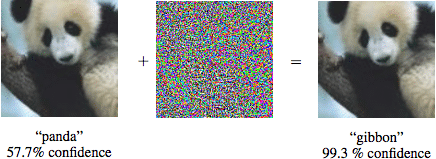
\includegraphics[width= 0.8\linewidth]{img/panda_ExAdvEx.png}

\footnote{\tiny Ian J. Goodfellow, Jonathon Shlens, and Christian Szegedy. Explaining and harnessing	adversarial examples. In 3rd International Conference on Learning Representations, ICLR 2015, San Diego, CA, USA, May 7-9, 2015, Conference Track Proceedings, 2015.}
\end{figure}
\end{frame}

%Nowadays we have enough knowledge about the capacity of machine learning models to make good predictions in different domains, like image classification, speech recognition, market analysis and image segmentation.
%The fundamental key point is that they are completely data-driven, they learn functions from data, and data contains noise by nature. In recent years researches discovered that these models are even sensitive to adversarial noise that can be deviced by malicious users. The greatest part of the works deal with supervised applications like in the following case in which by simply injecting a human-eyes imperceptible noise an attacker can subvert the original prediction from a panda to a gibbon.

 
\section{Unsupervised Learning}
\begin{frame}
  \frametitle{Clustering  Applications}
  \changefontsizes{8.5pt}
  %However, even unsupervised models are used in sophisticated applications and one of the main application of these models is clustering. The clustering analysis is the task of grouping a set of objects in such a way that objects in the same group (called a cluster) are more similar (in some sense) to each other than to those in other groups (clusters). Clustering is assuming a fundamental role in common application, due to the absence of labeled data. Some examples of applications could be ....
  % Despite their strong usage in sensitive application only few works have been done in this domain. A recent work proposed by Biggio et al proposed a framework for fooling hierarchical clustering, but it has not been develop for working against general clustering algorithms. In this thesis we developed 3 adversarial algorithms for fooling clustering algorithms in different applications.
  \begin{itemize}
  	\item Clustering is finding a wide range of applications, due to the absence of labeled data
  	\item Ex: Image segmentation, face clustering, market, social or crime analysis, malicious software clustering, information processing, etc.
  	
  	\begin{figure}
  		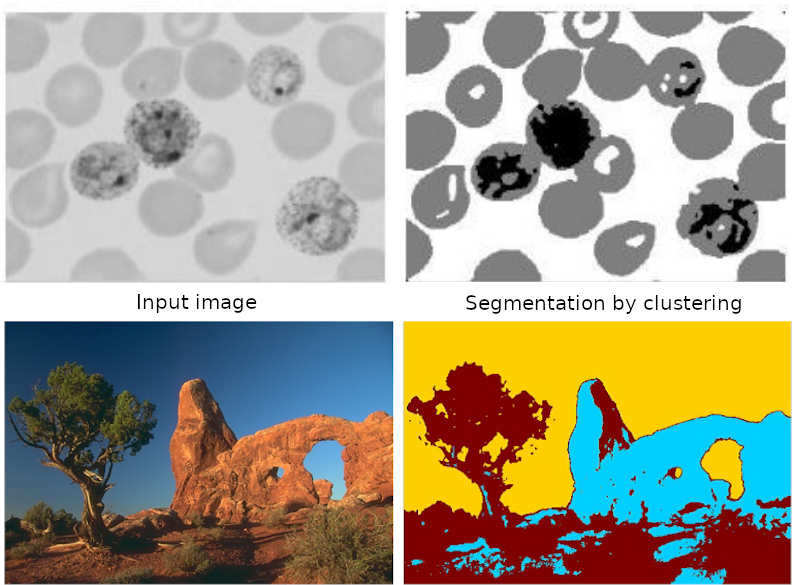
\includegraphics[width= 0.4\linewidth]{img/segmentation2.png}
  		
  		\footnote{\tiny Nameirakpam Dhanachandra, Khumanthem Manglem, Yambem Jina Chanu,
Image Segmentation Using K -means Clustering Algorithm and Subtractive Clustering Algorithm,
Procedia Computer Science.
  	}
  	\end{figure}
  	
  	\item Biggio et al. proposed a framework for fooling hierarchical clustering
  \end{itemize}
\end{frame}


\begin{frame}
	\frametitle{K-Means Clustering}
	% we decided to compare the robustness of three clustering algorithms. The first one is K-Means, which basically is a very well-known iterative and partition-based algorithm. It tries to resolve the clustering problem by maximizing a certain objective function which represent the cohesiveness of clusters. 
	% K-Means requires the knowledge of the number of clusters $K$ and from that it generates K centroids. Iteration by iteration it assigns samples to the cluster with the closest centroid and update the cluster centroids.
	% The fundamental issues of K-Means are that it can't handle non-convex set and it is sensitive to centroids initializations.
	\changefontsizes{8.pt}
	\begin{itemize}
		\item It splits $n$ objects into $K$ maximal cohesive groups by minimizing: \begin{scriptsize}
			$$\arg \min_C\sum_{i=0}^K \Biggl\{ \sum_{j \in \text{elements of } C_i\text{ cluster}} ||x_j - \mu_i||^2 \Biggr\}$$
		\end{scriptsize}
	%basically want to find the centroids that maximize the cohesiveness 
		where $\mu_i$ is the centroid of cluster $i$
		\item It is a polynomial algorithm that guaranteed to converge in a finite number of steps
		
	\end{itemize}
	\begin{block}{K-Means Algorithm}
		\begin{enumerate}
			
			\item Initialize cluster centroids $\mu_1, \dots, \mu_k,$.
			\item Repeat until all points remain unchanged (convergence):
			
			\begin{enumerate}
				\item Assign samples to clusters:  $\forall i\in X \quad c^{(i)} = \arg\min_j \vert\vert x^{(i)}-\mu_j\vert\vert^2$
				\item Update cluster centroids:  $\forall j\in C \quad \mu_j = \frac{\sum_{i=1}^m 1\{c^{(i)} = j\}x^{(i)}}{\sum_{i=1}^m 1\{c^{(i)} = j\}}$
			\end{enumerate}
		\end{enumerate}
	\end{block}
	\begin{itemize}
		\item Sensitive to cluster centroids initialization and can't handle non-convex set.
	\end{itemize}

\end{frame}

\begin{frame}
	\frametitle{Spectral Clustering}
	% The second clustering algorithm is Spectral clustering, which basically use but into another embedding space. Indeed, it uses properties of eigenvalues and eigenvectors for mapping samples from the original space to a spectral one, in which commonly clusters are more evident. Then, it uses K-Means over the new projection, allowing to cluster objects that are connected but not necessary within convex boundaries.
	\changefontsizes{8.pt}
	\begin{itemize}
		\item Uses properties of eigenvalues and eigenvectors for solving the clustering problem
\end{itemize}
\begin{block}{Spectral Clustering Algorithm}
\begin{enumerate}
	\begin{footnotesize}
		\item Construct a similarity graph and compute the normalized graph Laplacian $L_{sym}$.
		\item Embed data points in a low-dimensional space (spectral embedding), in which the clusters are more obvious, computing the $k$ smallest eigenvectors $v_1, \dots, v_k$ of $L_{sym}$. 
		\item Let $V=\left[v_1,\dots, v_k \right] \in \mathbb{ R }^{n \times k}$.
		\item Form the matrix $U \in \mathbb{ R }^{n \times k}$ from $V$ by normalizing the row sums to have norm 1, that is: 
		
		$$u_ { i j } = \frac { v _ { i j } } { \left( \sum _ { k } v _ { i k } ^ { 2 } \right) ^ { 1 / 2 } }$$
		\item For $i=1,\dots, n$, let $y _ { i } \in \mathbb { R } ^ { k }$ be the vector corresponding to the $i$th row of $U$.
		\item Cluster the points $y_i$ with $i=1,\dots,n$ with the $k$-means algorithm into clusters $C_1, \dots, C_k$.
	\end{footnotesize}
\end{enumerate}
\end{block}
\begin{itemize}
	\item Applying K-Means on the spectral embedding allows to cluster objects that are connected but not necessarily compact or clustered within convex boundaries.
\end{itemize}
\end{frame}

\begin{frame}
	\frametitle{Dominant Sets Clustering}
	\changefontsizes{8.pt}
	\begin{itemize}
	\item Graph-theory based approach supported by game theory
	\item Clusters correspond to dominant sets
	\item Implemented using deterministic game dynamics like discrete Replicator Dynamics
	\item Robust against noise, allows to find overlapped clusters, makes no assumptions on the similarity matrix and on the number of clusters
	%RICORDARSI CHE SPECTRAL RICHIEDE CHE LA MATRICE SIA SIMMETRICA
\end{itemize}
	\begin{block}{Extract a dominant set}
	\begin{footnotesize}
	\begin{enumerate}
		\item distance = $\infty$
		\item while distance $> \varepsilon$:
		\begin{enumerate}
			\item $x_i(t+1) = x_i(t)\frac{(Ax(t))_i}{x(t)^TAx(t)}$
			\item distance = \texttt{norm}($x_i(t+1) - x_i(t)$)
		\end{enumerate}
		\item return $\sigma(x)$
	\end{enumerate}
	\end{footnotesize}
\end{block}

	\begin{block}{Dominant Sets Algorithm}
	\begin{footnotesize}
	\begin{enumerate}
		\item Extract all dominant sets or $K$ of them from the input similarity matrix
	\end{enumerate}
	\end{footnotesize}
	\end{block}
\end{frame}

\section{Adversarial Algorithms}

\begin{frame}
  \frametitle{Rows-based Adversarial Generator}
  	\changefontsizes{8.pt}
	\begin{itemize}
		\item Fooling image segmentation systems using rows-based noise
		\item Optimization is done using a genetic algorithm
	\end{itemize}
	\begin{block}{Rows-based Adversarial Generator Algorithm}

		\begin{enumerate}
			\item Pick $s$ most sensitive rows in input $X$
			\item For each $p$-consecutive pixels in each row find the optimal adversarial noise $\varepsilon^*$ to inject.
			\begin{itemize}
				\item \textbf{Objective function}: distance or dissimilarity from the initial segmentation. 
	
				\item Maximum adversarial perturbation level $\Delta$.
				
				\item Generate a random perturbation $\varepsilon$ to inject. Evaluate the fitness function and apply stochastic operators for improving $\varepsilon$.
			\end{itemize}
			\item Craft adversarial example: $X^\prime\rightarrow X + \varepsilon^*$
		\end{enumerate}

	\end{block}
\end{frame}



\begin{frame}
	\frametitle{Rows-based Adversarial Generator}
	\changefontsizes{6.pt}

\begin{figure}[H]
	\begin{minipage}[t]{0.3\linewidth}
		\centering
		
\includegraphics[width=0.8\textwidth]{img/advrows/5.png}
		\caption{\small Input digit X from MNIST.}
	\end{minipage}        
	\hspace{.1cm}
	\begin{minipage}[t]{0.3\linewidth}
		\centering
		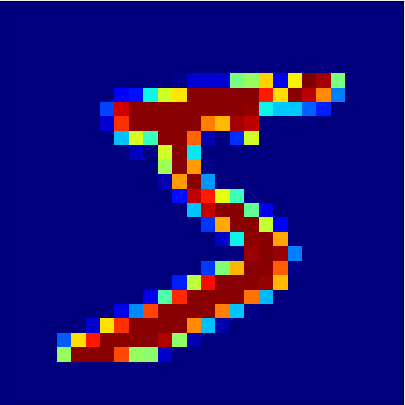
\includegraphics[width=0.8\textwidth]{img/advrows/5jet.png}
		\caption{\small Jet visualization of $X$.}
	\end{minipage}
	\hspace{.1cm}
	\begin{minipage}[t]{0.3\linewidth}
		\centering
		
\includegraphics[width=0.8\textwidth]{img/advrows/5y.png}
		\caption{\small Spectral Clustering predicted segmentation.}
	\end{minipage}
\end{figure}

\begin{figure}[H]
	\begin{minipage}[t]{0.3\linewidth}
		\centering
		
\includegraphics[width=0.8\textwidth]{img/advrows/5adv.png}
			\caption{\small Adversarial digit $X^\prime$.}
	\end{minipage}        
	\hspace{.1cm}
	\begin{minipage}[t]{0.3\linewidth}
		\centering
		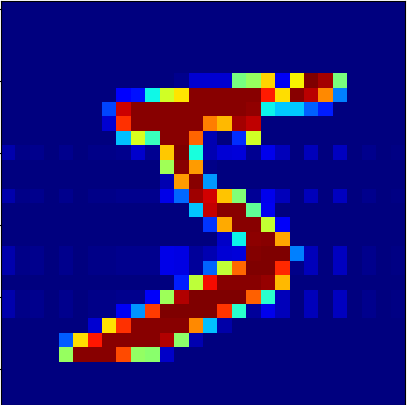
\includegraphics[width=0.8\textwidth]{img/advrows/5advjet.png}
		\caption{\small Jet visualization of $X^\prime$.}
	\end{minipage}
	\hspace{.1cm}
	\begin{minipage}[t]{0.3\linewidth}
		\centering
		
\includegraphics[width=0.8\textwidth]{img/advrows/5advy.png}
		\caption{\small Spectral Clustering adversarial segmentation.}
	\end{minipage}
\end{figure}
\end{frame}

\begin{frame}
	\frametitle{Pixel-wise Adversarial Generator}
	\changefontsizes{8.pt}
	\begin{itemize}
		\item Fooling image segmentation systems using pixel-wise noise
		\item Injected noise seems to be random (like gaussian or salt-and-pepper)
		\item Adversarial noise is targeted and attack sensitive regions
	\end{itemize}
	\begin{block}{Pixel-wise Adversarial Generator Algorithm}
		
		\begin{enumerate}
			\item Pick $s$ most sensitive pixels in input $X$
			\item For each $p$-consecutive sensitive pixels find the optimal adversarial noise $\varepsilon^*$ to inject.
			\begin{itemize}
				\item \textbf{Objective function}: distance or dissimilarity from the initial segmentation. 
				
				\item Maximum adversarial perturbation level $\Delta$.
				
				\item Generate a random perturbation $\varepsilon$ to inject. Evaluate the fitness function and apply stochastic operators for improving $\varepsilon$.
			\end{itemize}
			\item Craft adversarial example: $X^\prime\rightarrow X + \varepsilon^*$
		\end{enumerate}
		
	\end{block}
\end{frame}


\begin{frame}
	\frametitle{Pixel-wise Adversarial Generator}
	\changefontsizes{6.pt}
	
	\begin{figure}[H]
		\begin{minipage}[t]{0.3\linewidth}
			\centering
			
\includegraphics[width=0.75\textwidth]{img/advpixel/example.png}
			\caption{\small Input digit X from MNIST.}
		\end{minipage}        
		\hspace{.1cm}
		\begin{minipage}[t]{0.3\linewidth}
			\centering
			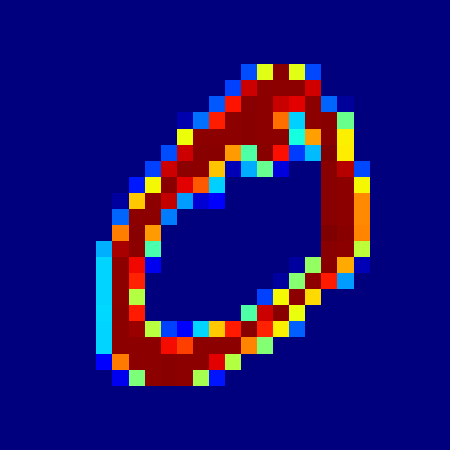
\includegraphics[width=0.75\textwidth]{img/advpixel/examplejet.png}
			\caption{\small Jet visualization of $X$.}
		\end{minipage}
		\hspace{.1cm}
		\begin{minipage}[t]{0.3\linewidth}
			\centering
			
\includegraphics[width=0.75\textwidth]{img/advpixel/predicted.png}
			\caption{\small Dominant Sets predicted segmentation.}
		\end{minipage}
	\end{figure}
	
	\begin{figure}[H]
		\begin{minipage}[t]{0.3\linewidth}
			\centering
			
\includegraphics[width=0.75\textwidth]{img/advpixel/xadv.png}
			\caption{\small Adversarial digit $X^\prime$.}
		\end{minipage}        
		\hspace{.1cm}
		\begin{minipage}[t]{0.3\linewidth}
			\centering
			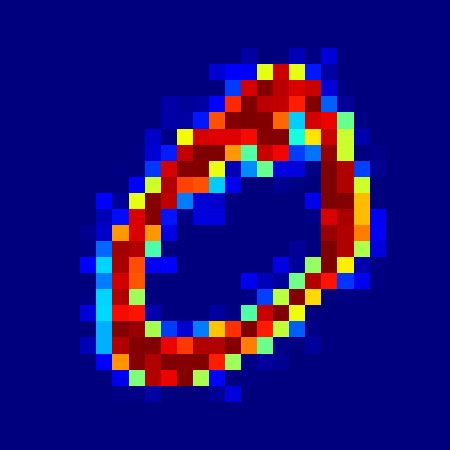
\includegraphics[width=0.75\textwidth]{img/advpixel/advjet.png}
			\caption{\small Jet visualization of $X^\prime$.}
		\end{minipage}
		\hspace{.1cm}
		\begin{minipage}[t]{0.3\linewidth}
			\centering
			
\includegraphics[width=0.75\textwidth]{img/advpixel/advpredicted.png}
			\caption{\small Dominant Sets adversarial segmentation.}
		\end{minipage}
	\end{figure}
\end{frame}


\begin{frame}
	\frametitle{Target Clustering Adversarial Generator}
  	\changefontsizes{8.pt}
	\begin{itemize}
		\item Fooling feature-based data clustering systems
		\item The attacker aims to break partially the resulting clusters composition
		\item Sensitive or target samples are moved towards a target cluster
	\end{itemize}
	\begin{block}{Rows-based Adversarial Generator Algorithm}
		
		\begin{enumerate}
			\item Pick $s$ most sensitive samples from input $X$
			\item For each $p$-consecutive features find the optimal adversarial noise $\varepsilon^*$ to inject for moving samples from a cluster towards a desired one.
			\begin{itemize}
				\item \textbf{Objective function}: distance or dissimilarity from the initial cluster labeling. 
				
				\item Maximum adversarial perturbation level $\Delta$.
				
				\item Generate a random perturbation $\varepsilon$ to inject. Evaluate the fitness function and apply stochastic operators for improving $\varepsilon$.
			\end{itemize}
			\item Craft adversarial example: $X^\prime\rightarrow X +  \varepsilon^*$
		\end{enumerate}
	\end{block}
\end{frame}


\section{Experiments}

\begin{frame}
  \frametitle{Experimental Setup}
   	\changefontsizes{8.pt}
  \begin{itemize}
  	\item Segmentation dataset: MNIST 
  	\item Clustering datasets: Synthetic, Yale Face, DIGITS
  	\item No initialization effect is introduced (multiple iterations with different seeds)
  	
  	\item $ARI$\footnote{\tiny Glenn Milligan and Martha Cooper. A study of the comparability of external criteria for
  		hierarchical cluster-analysis. Multivariate Behavioral Research - MULTIVARIATE BEHAV
  		RES, 21:441–458, 10 1986. doi: 10.1207/s15327906mbr2104 5.}
  	 and $ARI_h$, as proposed by Milligan et al.,for analyzing clustering quality
  	 %The Rand Index computes a similarity measure between two clusterings by considering all pairs of samples and counting pairs that are assigned in the same or different clusters in the predicted and true clusterings.
  	
  	\item $\vert \vert X - X^\prime\vert \vert_2$\footnote{\tiny{Battista Biggio, Ignazio Pillai, Samuel Rota Bulò, Davide Ariu, Marcello Pelillo, and Fabio
  			Roli. Is data clustering in adversarial settings secure? In AISec’13, Proceedings of the 2013
  			ACM Workshop on Artificial Intelligence and Security, Co-located with CCS 2013, Berlin,
  			Germany, November 4, 2013, pages 87–98, 2013.}}, as suggested by Biggio et al., for representing the attacker's capacity
  	\item Gaussian Similarity is used for constructing the similarity matrix
  	$$A(i,j) = \exp\Big(\frac{-\vert\vert\psi(i)- \psi(j)\vert\vert_2^2}{2\sigma^2}\Big)$$
  \end{itemize}

\end{frame}

\begin{frame}
	\frametitle{Rows-based Results}
   	\changefontsizes{7.pt}
	\begin{figure}[H]
		\begin{minipage}[t]{0.48\linewidth}
			\centering
			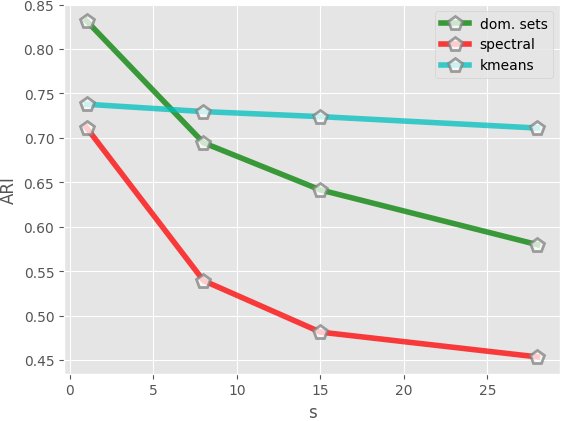
\includegraphics[width=0.65\textwidth]{img/advrows/rows_ARI.png}
			\caption{\footnotesize $ARI$ over number of perturbed rows $s$.}
		\end{minipage}        
		\hspace{.1cm}
		\begin{minipage}[t]{0.48\linewidth}
			\centering
			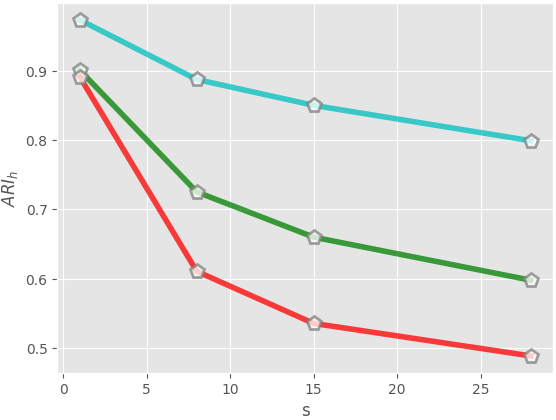
\includegraphics[width=0.65\textwidth]{img/advrows/rows_ARIh.png}
			\caption{\footnotesize $ARI_h$ over number of perturbed rows $s$.}
		\end{minipage}
	\end{figure}

	\begin{figure}[H]
	\begin{minipage}[t]{0.45\linewidth}
		\centering
		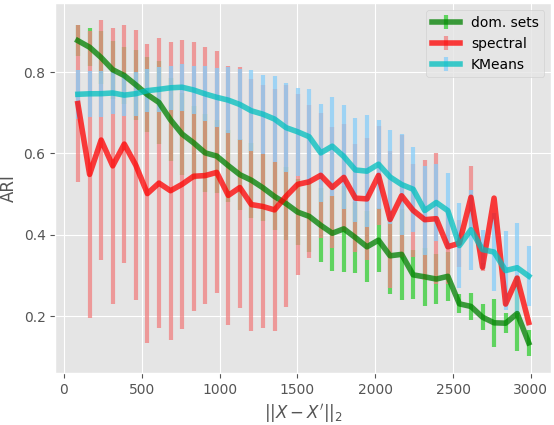
\includegraphics[width=0.65\textwidth]{img/advrows/X2_ARI.png}
		\caption{\footnotesize $ARI$ over attacker's capacity $\vert \vert X - X^\prime\vert \vert_2$.}
	\end{minipage}        
	\hspace{.1cm}
	\begin{minipage}[t]{0.45\linewidth}
		\centering
		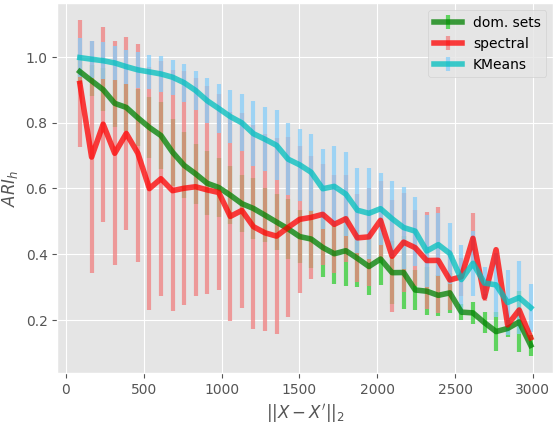
\includegraphics[width=0.65\textwidth]{img/advrows/X2_ARIh.png}
		\caption{\footnotesize $ARI_h$ over attacker's capacity $\vert \vert X - X^\prime\vert \vert_2$.}
	\end{minipage}
\end{figure}
   	\changefontsizes{7.8pt}
\begin{itemize}
	\item High sensitivity of Spectral Clustering to the number of attacked rows $s$
	\item Greater robustness provided by Dominant Sets and K-Means
\end{itemize}
\end{frame}

\begin{frame}
	\frametitle{Pixel-wise Results}
   	\changefontsizes{7.pt}
\begin{figure}[H]
	\begin{minipage}[t]{0.48\linewidth}
		\centering
		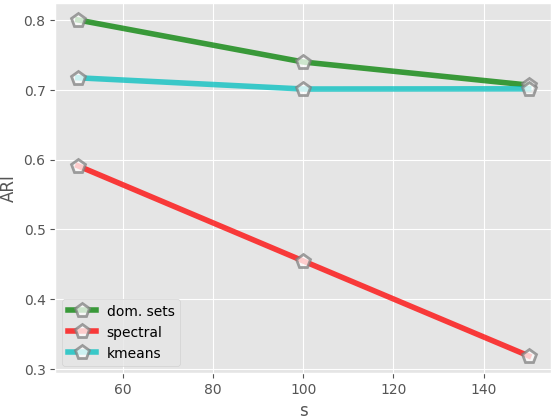
\includegraphics[width=0.65\textwidth]{img/advpixel/rows_ARI.png}
		\caption{\footnotesize $ARI$ over number of perturbed pixels $s$.}
	\end{minipage}        
	\hspace{.1cm}
	\begin{minipage}[t]{0.48\linewidth}
		\centering
		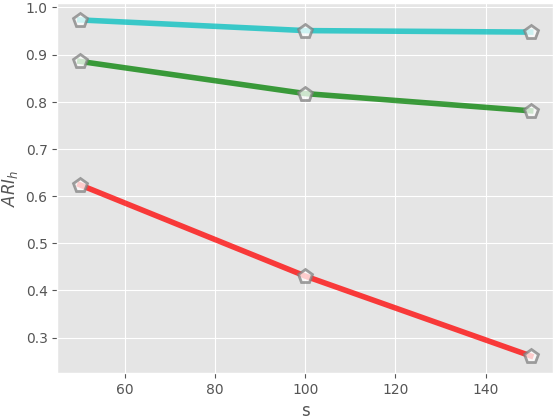
\includegraphics[width=0.65\textwidth]{img/advpixel/rows_ARIh.png}
		\caption{\footnotesize $ARI_h$ over number of perturbed pixels $s$.}
	\end{minipage}
\end{figure}

\begin{figure}[H]
	\begin{minipage}[t]{0.45\linewidth}
		\centering
		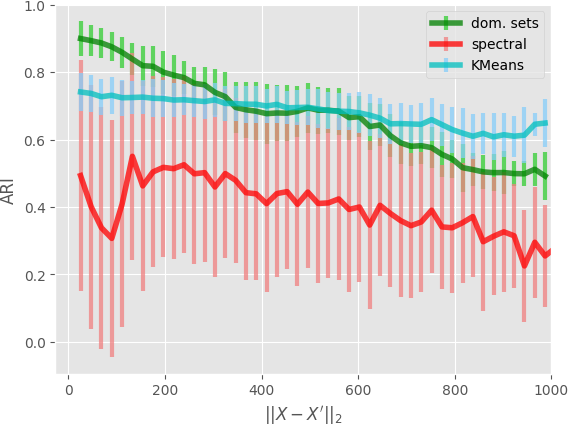
\includegraphics[width=0.65\textwidth]{img/advpixel/X2_ARI.png}
		\caption{\footnotesize $ARI$ over attacker's capacity $\vert \vert X - X^\prime\vert \vert_2$.}
	\end{minipage}        
	\hspace{.1cm}
	\begin{minipage}[t]{0.45\linewidth}
		\centering
		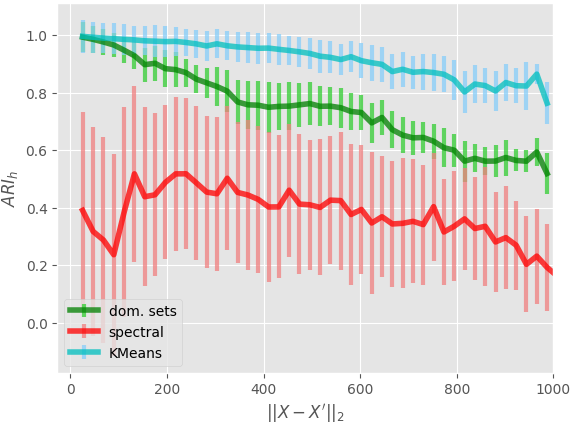
\includegraphics[width=0.65\textwidth]{img/advpixel/X2_ARIh.png}
		\caption{\footnotesize $ARI_h$ over attacker's capacity $\vert \vert X - X^\prime\vert \vert_2$.}
	\end{minipage}
\end{figure}
\changefontsizes{7.8pt}
\begin{itemize}
	\item High sensitivity of Spectral Clustering to the number of attacked pixels $s$
	\item Greater robustness provided by Dominant Sets and K-Means
\end{itemize}
\end{frame}




\begin{frame}
	\frametitle{Target Clustering Results - Synthetic}
	   	\changefontsizes{7.pt}
	   	
	\begin{figure}[H]
   		\begin{minipage}[t]{0.45\linewidth}
   			\centering
   			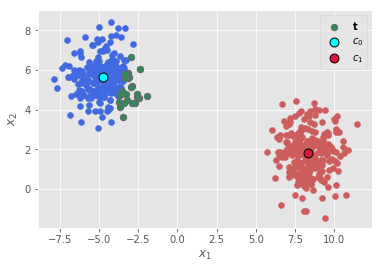
\includegraphics[width=0.9\textwidth]{img/target/XsyntheticTargets.png}
   			\caption{\footnotesize Synthetic dataset and target samples (green).}
   		\end{minipage}        
   		\hspace{.1cm}
   		\begin{minipage}[t]{0.45\linewidth}
   			\centering
   			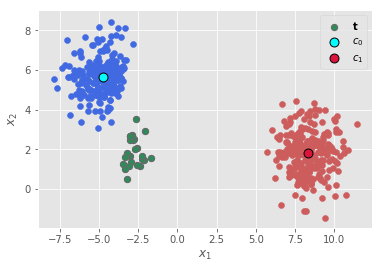
\includegraphics[width=0.9\textwidth]{img/target/XsyntheticAdv.png}
   			\caption{\footnotesize Adversarial samples $X^\prime$.}
   		\end{minipage}
   	\end{figure}
	\begin{figure}[H]
		\begin{minipage}[t]{0.30\linewidth}
			\centering
			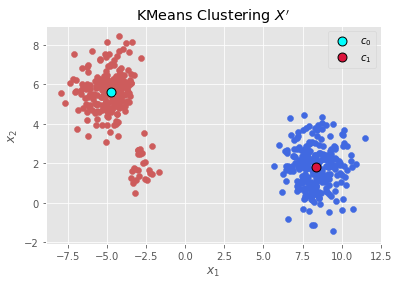
\includegraphics[width=1\textwidth]{img/target/kmeansXadv.png}
		\end{minipage}        
		\hspace{.1cm}
		\begin{minipage}[t]{0.30\linewidth}
			\centering
			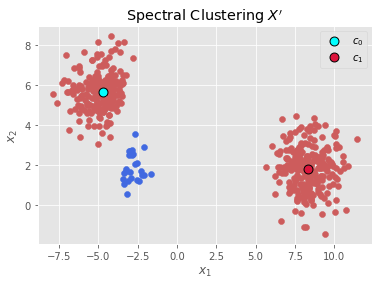
\includegraphics[width=1\textwidth]{img/target/spectralXadv.png}
		\end{minipage}
		\hspace{.1cm}
		\begin{minipage}[t]{0.30\linewidth}
		\centering
		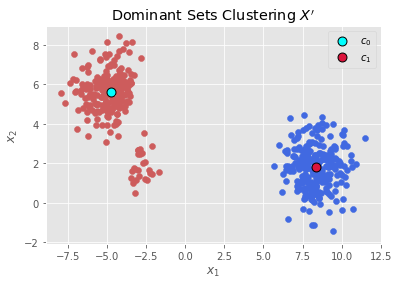
\includegraphics[width=1\textwidth]{img/target/dominantXadv.png}
	\end{minipage}
	\caption{\footnotesize Data clustering obtained for X 0 using K-Means (left), Spectral (middle) and Dominant Sets (right) clustering.}
	\end{figure}
	
\end{frame}

\begin{frame}
	\frametitle{Target Clustering Results - Synthetic}
	\changefontsizes{7.pt}
		\begin{figure}[H]
		\begin{minipage}[t]{0.45\linewidth}
			\centering
			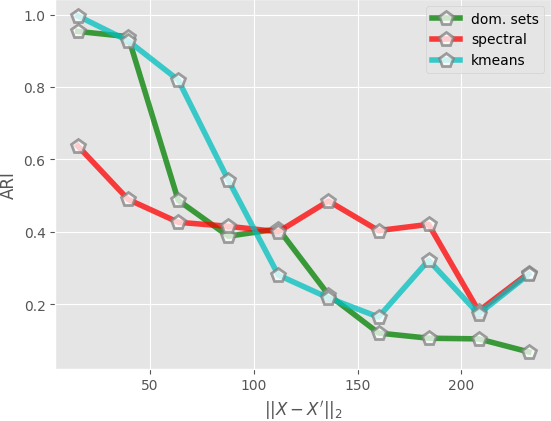
\includegraphics[width=1\textwidth]{img/target/X2_ARI.png}
			\caption{\footnotesize $ARI$ over attacker's capacity  $\vert \vert X - X^\prime\vert \vert_2$.}
		\end{minipage}        
		\hspace{.1cm}
		\begin{minipage}[t]{0.45\linewidth}
			\centering
			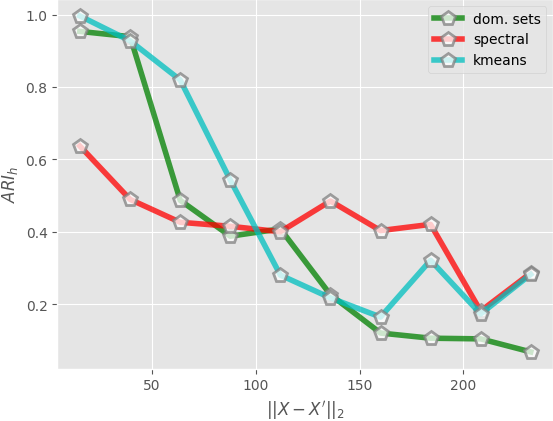
\includegraphics[width=1\textwidth]{img/target/X2_ARIh.png}
			\caption{\footnotesize $ARI_h$ over attacker's capacity $\vert \vert X - X^\prime\vert \vert_2$.}
		\end{minipage}
	\end{figure}
	\changefontsizes{8pt}
\begin{itemize}
	\item High sensitivity of Spectral Clustering to small perturbations
	\item Spectral embedding affected by adversarial noise
	\item Greater robustness provided by K-Means and Dominant Sets
\end{itemize}
\end{frame}



\begin{frame}
	\frametitle{Target Clustering Results - Yale Face}
	\changefontsizes{7.pt}
	
	\begin{figure}[H]
		\begin{minipage}[t]{0.45\linewidth}
			\centering
			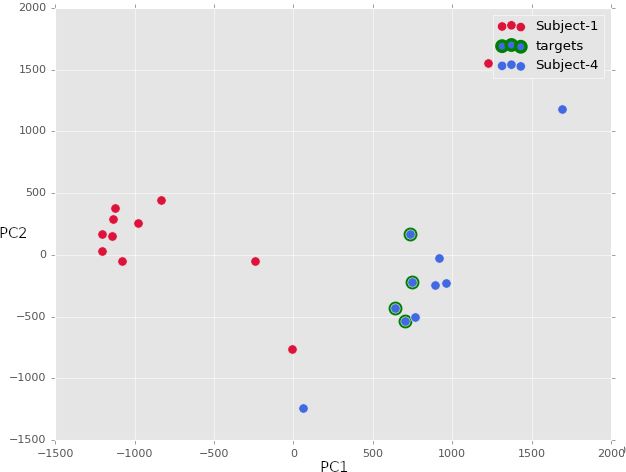
\includegraphics[width=0.9\textwidth]{img/target/pcaYale.png}
			\caption{\footnotesize Yale Face subject-1 and subject-4 clusters with 2-PC projection. Target samples are highlighted in green.}
		\end{minipage}        
		\hspace{.1cm}
		\begin{minipage}[t]{0.45\linewidth}
			\centering
			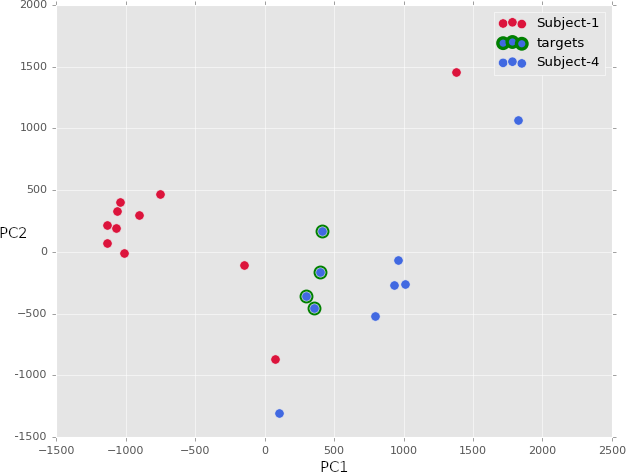
\includegraphics[width=0.9\textwidth]{img/target/pcaYaleadv.png}
			\caption{\footnotesize Adversarial Yale Face dataset $X^\prime$ with 2-PC projection.}
		\end{minipage}
	\end{figure}
	\begin{figure}[H]
		\begin{minipage}[t]{0.30\linewidth}
			\centering
			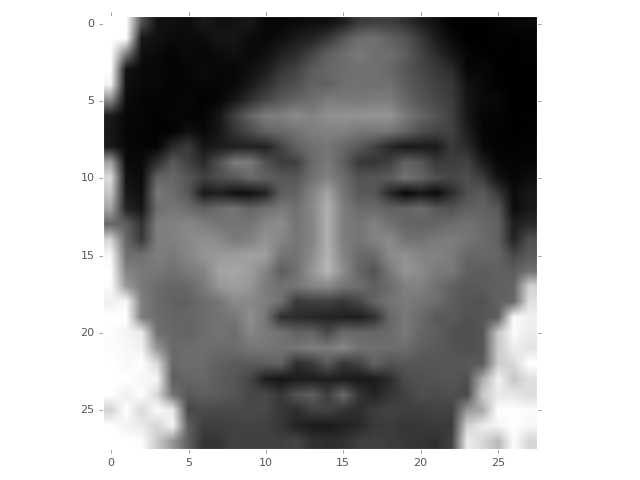
\includegraphics[width=0.95\textwidth]{img/target/subject0.png}
		\end{minipage}        
		\hspace{.1cm}
		\begin{minipage}[t]{0.30\linewidth}
			\centering
			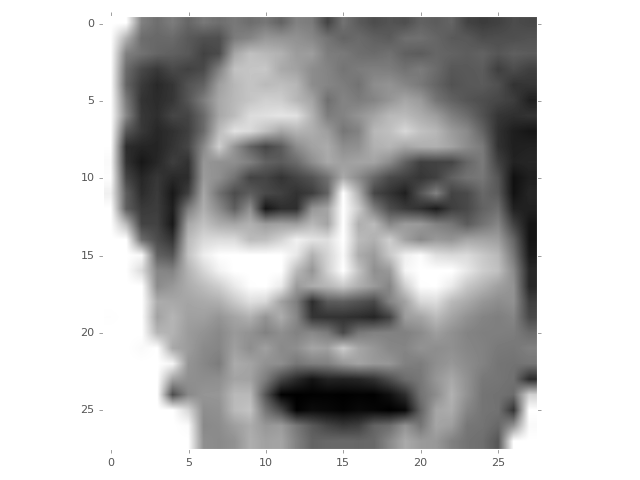
\includegraphics[width=0.95\textwidth]{img/target/targetface.png}
		\end{minipage}
		\hspace{.1cm}
		\begin{minipage}[t]{0.30\linewidth}
			\centering
			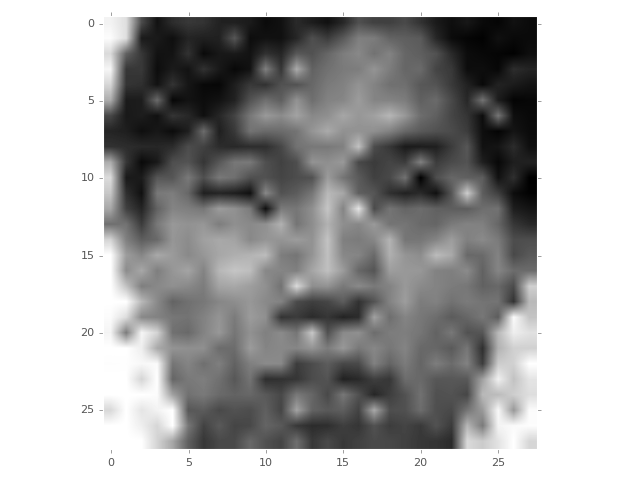
\includegraphics[width=0.95\textwidth]{img/target/advsubject0.png}
		\end{minipage}
		\caption{\footnotesize Sample in subject-4 on the right moved towards subject-1 cluster (sample on the middle). The crafted adversarial examples in shown on the right.}
	\end{figure}
	
\end{frame}

\begin{frame}
	\frametitle{Target Clustering Results - Yale Face}
	\changefontsizes{7.pt}
	\begin{figure}[H]
		\begin{minipage}[t]{0.45\linewidth}
			\centering
			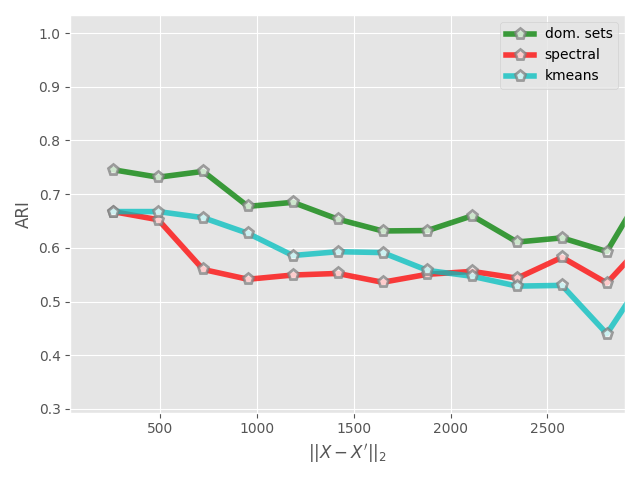
\includegraphics[width=1\textwidth]{img/target/yaleARI.png}
			\caption{\footnotesize $ARI$ over attacker's capacity  $\vert \vert X - X^\prime\vert \vert_2$.}
		\end{minipage}        
		\hspace{.1cm}
		\begin{minipage}[t]{0.45\linewidth}
			\centering
			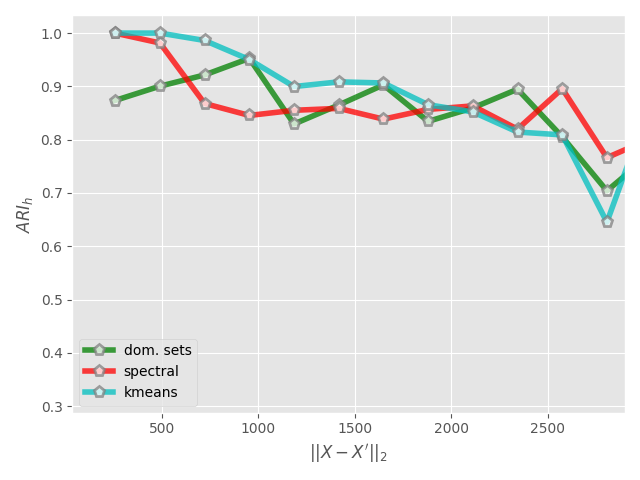
\includegraphics[width=1\textwidth]{img/target/yaleARIh.png}
			\caption{\footnotesize $ARI_h$ over attacker's capacity $\vert \vert X - X^\prime\vert \vert_2$.}
		\end{minipage}
	\end{figure}
	\changefontsizes{8pt}
	\begin{itemize}
		\item Even face clustering can be fooled
		\item The three algorithms react similarly in presence of adversarial noise
	\end{itemize}
\end{frame}


\section{Conclusions}

\begin{frame}
  \frametitle{Conclusions and Future Work}
  	\changefontsizes{8.5pt}
\textbf{Conclusions:}
  \begin{itemize}
  	\item Image segmentation and clustering algorithms are sensitive to adversarial noise. Defensive strategy are required.
    \item Dominant Sets seems to be robust even against adversarial noise
    \item Spectral Clustering seems to be strongly sensitive to small adversarial perturbations.\\
  \end{itemize}
\vspace{0.7cm}
\textbf{Future work:}
	\begin{itemize}
		\item Speed up the adversarial algorithms using GPUs architectures
		\item Consider different similarity measures and embedding
		\item Generalize the adversarial target clustering to $k$ clusters
		\item Evaluate an outlier detection analysis over crafted adversarial examples
	\end{itemize}
\end{frame}



\section{Bibliography}

\begin{frame}
	\frametitle{Bibliography}
	\changefontsizes{6.5pt}
	\begin{itemize}
		\item {{Battista Biggio and Fabio Roli. Wild patterns: Ten years after the rise of adversarial
		machine learning. In Proceedings of the 2018 ACM SIGSAC Conference on Computer and
		Communications Security, CCS 2018, Toronto, ON, Canada, October 15-19, 2018, pages
		2154–2156, 2018.}}\\
	
	
		\item {{Battista Biggio, Ignazio Pillai, Samuel Rota Bulò, Davide Ariu, Marcello Pelillo, and Fabio
				Roli. Is data clustering in adversarial settings secure? In AISec’13, Proceedings of the 2013
				ACM Workshop on Artificial Intelligence and Security, Co-located with CCS 2013, Berlin,
				Germany, November 4, 2013, pages 87–98, 2013.}}\\
			
		\item {{Massimiliano Pavan and Marcello Pelillo. Dominant sets and pairwise clustering. IEEE
				Transactions on Pattern Analysis and Machine Intelligence, 29:167–172, 2007.}}\\
			
		\item {{Ulrike von Luxburg. A tutorial on spectral clustering. Statistics and Computing, 17(4):
				395–416, 2007.}}
			
		\item {{Christopher M. Bishop. 2006. Pattern Recognition and Machine Learning (Information Science and Statistics). Springer-Verlag, Berlin, Heidelberg.
		}}
	\end{itemize}
\end{frame}

\end{document}
